% Search for all the places that say "PUT SOMETHING HERE".

\documentclass[11pt]{article}
\usepackage{textcomp,graphicx,enumerate}
\usepackage{proof}
\usepackage{diagbox}
\usepackage{algorithmicx}  
\usepackage{subcaption}
\def\Name{Yingkun Zhou}  % Your name
\def\Email{zhouyingkun15@mails.ucas.ac.cn}
\title{The Tale of Alpha Series Microprocessor}
\author{\Name \\ \Email}
\pagestyle{myheadings}


\newenvironment{qparts}{\begin{enumerate}[{(}a{)}]}{\end{enumerate}}
\def\endproofmark{$\Box$}
\newenvironment{proof}{\par{\bf Proof}:}{\endproofmark\smallskip}

\textheight=9in
\textwidth=6.5in
\topmargin=-.75in
\oddsidemargin=0.25in
\evensidemargin=0.25in
\usepackage[procnames]{listings}

\usepackage{amssymb} % needed for math
\usepackage{amsmath} % needed for math
\usepackage[utf8]{inputenc} % this is needed for german umlauts
\usepackage[ngerman,english]{babel} % this is needed for german umlauts
\usepackage[T1]{fontenc}    % this is needed for correct output of umlauts in pdf
\usepackage[margin=2.5cm]{geometry} %layout
\usepackage{listings} % needed for the inclusion of source code

% the following is needed for syntax highlighting
\usepackage{color}
\definecolor{keywords}{RGB}{255,0,90}
\definecolor{comments}{RGB}{0,0,113}
\definecolor{red}{RGB}{160,0,0}
\definecolor{green}{RGB}{0,150,0}
\makeatletter
\newcommand{\rmnum}[1]{\romannumeral #1}
\newcommand{\Rmnum}[1]{\expandafter\@slowromancap\romannumeral #1@}
\makeatother
\lstset{language=Python, 
	basicstyle=\ttfamily\small, 
	keywordstyle=\color{keywords},
	commentstyle=\color{comments},
	stringstyle=\color{red},
	showstringspaces=false,
	identifierstyle=\color{green},
	procnamekeys={def,class}}

% this is needed for forms and links within the text
\usepackage{hyperref}
\newcommand{\note}[1]{\scriptsize{#1}\normalsize}
\newcommand{\emphasize}[1]{\huge{#1}\normalsize}
\begin{document}
\maketitle

In the current stage, I want to focus the tech of designing high performance uniprocessor based on my latest knowledge, as a senior undergraduate student. Though I know that a computer system nowadays is far away from a powerful uniprocessor. It means that we not only need to fully explore parallelism and thus introduce multiprocessor, but also means that but also need to develop full-featured software environment which can run in our ISA, which is considered as the most important aspect. Intel and DEC are the pair of such example. In 1990s, DEC has the most powerful microprocessor--Alpha series at that time, with peak frequency up to 600MHz, 64 bits architecture, 4-issue, 80-instruction execution at same time, while Intel's fastest microprocessor--Pentium II only has 300MHz peak frequency with 32 bits, poorly designed architecture and the worst ISA. Ironically, Intel survived while DEC dead, quite funny history. But, anyway, as a milestone in the microprocessor history, the tech reflected in the Alpha design still worth learning, especially for me, who wants to design self high performance CPU (based on RISC-V ISA maybe).   

\renewcommand{\labelenumi}{\Roman{enumi}}
\section*{1.low digit circuit aspect\footnote{reading note from \textit{High-performance Microprocessor}}}
There are there generation of Alpha microprocessors. Following is the features.
\begin{itemize}
	\item 21064: $1.68\times10^6$ transistors, 200MHz, .75$ \mu $m n-well CMOS process, 16 gate delays/cycle, 3.3V, 30W
	\item 21164: $9.3\times10^6$ transistors, 300MHz, .50$ \mu $m n-well CMOS process, 14 gate delays/cycle, 3.3V, 50W
	\item 21264: $1.52\times10^7$ transistors, 600MHz, .35$ \mu $m n-well CMOS process, 12 gate delays/cycle, 2.2V, 72W
\end{itemize}
Some features of the Alpha ISA:
\renewcommand{\labelenumi}{\roman{enumi}}
\begin{enumerate}
	\item 64-bit lw/sw RISC arch 
	\item Fix-length instructions
	\item minimal instruction ordering constraints
	\item 64-bit manipulation allow for straightforward instruction decode (\textbf{confused}) 
	\item does not contain condition codes (like x86), branch delay slots (like MIPS), adaptations from existing 32-bit arch (\textbf{bad for Compatibility})
\end{enumerate}
CPU inner arch impl detail:
\begin{itemize}
	\item 21064: fully pipelined, in-order execution, 2-issue, one pipelined integer execution unit (\textbf{one or two cycles except for multiplies which are not pipelined}), one pipelined floating point execution unit (\textbf{6 cycles for all instructions except for divides}). 8KB Icache, 8KB Dcache
	\item 21164: quad-issue, in-order execution; contains 2 pipelined integer execution units (\textbf{one cycle for all integer instructions and roughly halved for all MUL instructions}), 2 pipelined floating-point execution units (separate add and multiply pipelines, 4-cycle latency); L1-level cache was changed to \textbf{nonblocking}; L2-level 96KB unified I and D cache.
	\item 21264: 6-way-issue and out-of-order execution; 4 integer execution units and 2 floating-point execution units; L1-Icache and L1-Dcache are both 64KB (eliminate on-chip L2 cache); reduce the divide latency by 50\% (extends to include square root and multimedia instructions)
\end{itemize}

The \Rmnum{3} part is confusing especially \textit{definition of Design Rules} thanks to my poor knowledge about the CMOS process field.
\newline

Circuit style highlight of Alpha series (\textbf{impl with a wide range of circuit styles including conventional complementary CMOS logic, single- and dual-rail dynamic logic, cascode logic pass transistor logic, and ratioed static logic}):
\begin{enumerate}
	\item full-custom circuit design methodologies. 
	\item Dynamic circuits: widely used in both data path and random control structures. The advantages are following:\\
	\begin{center}
		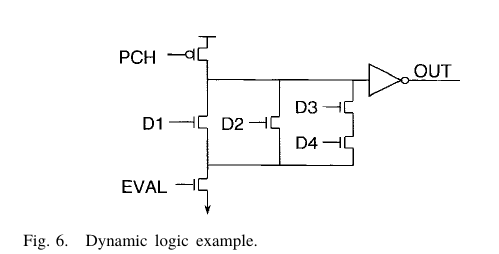
\includegraphics[scale=0.5]{dynamic.png}
	\end{center}
	\begin{enumerate}
		\item wide OR, no need many levels of complementary logic
		\item eliminating the PMOS transistor network reduces both the gate fan-int and fan-out capacitance. 
		\item the switching point of the dynamic gate is set by the NOMS device threshold voltage. (\note{if the timing of the inputs is such that they are not asserted until after the precharge clock has been deasserted, there in no crossover current during the output transition}) \textbf{a bit of confused}
		\item Removing the PMOS transistor network reduces the layout area, which results in lower interconnect capacitance, further increasing the speed of the circuit.
	\end{enumerate}
	\item dual-rail cascode logic, used in both data path and random control logic areas. The advantages are following:\\
	\begin{center}
		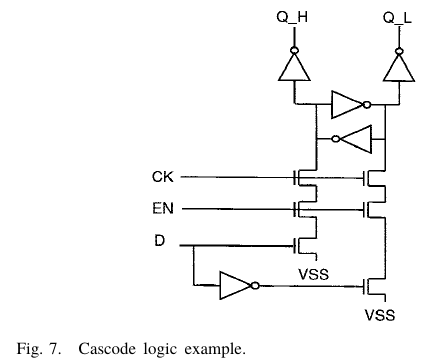
\includegraphics[scale=0.5]{cascode.png}	
	\end{center}
	\begin{enumerate}
		\item the fan-in and fan-out capacitance are both lower, thus reducing delay.
		\item Large complex functions such as multiplexers and XOR gates can be easily implemented in a single cascode gate with both true and complement outputs.
		\item a latch function can easily be constructed with addition of one pair of transistors.
	\end{enumerate}
\end{enumerate}

\textit{Power Dissipation and Supply Distribution} part is \textbf{quite confusing}. Again based on my poor knowledge cannot understand the analysis why to add aluminum interconnect layer(M3 lines), M4, and two thick low-resistance aluminum reference planes step by step to satisfy the limitation of power. Just put the graph here in case of need for discussing. \\
\begin{center}
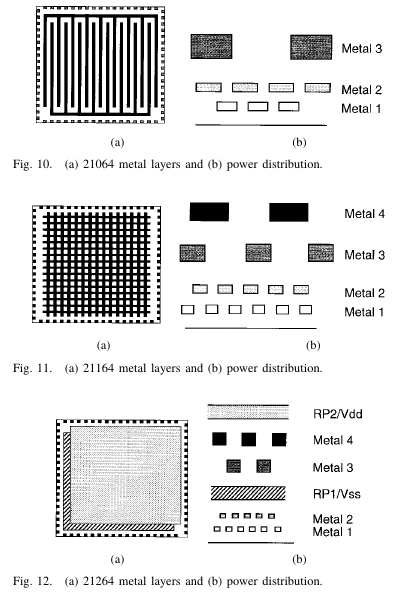
\includegraphics[scale=0.5]{layers.png} 
\end{center}

\textit{Clock Distribution}\\
The motivation of this part is that the high frequencies of the Alpha microprocessors have required the generation and distribution of a very high-quality clock signal and the use of fast (low-latency) latches. 

Here is the possible impact of clock system on the performance of the microprocessor:
\begin{itemize}
	\item Uncertainties in clock edges resulting form power supply noise, process variation and interconnect RC delay lower the maximum clock frequency of the microprocessor.
	\item slow clock edges introduce uncertainties in latch timing which further limit performance and can lead to functional failures due to latch race-through.
\end{itemize}
\begin{figure}[h]
	\centering
	\begin{subfigure}[b]{0.3\textwidth}
		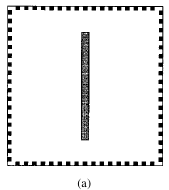
\includegraphics[width=\textwidth]{21064_1.png}
		\caption{clock driver location}
	\end{subfigure}
	~ %add desired spacing between images, e. g. ~, \quad, \qquad, \hfill etc. 
	%(or a blank line to force the subfigure onto a new line)
	\begin{subfigure}[b]{0.3\textwidth}
		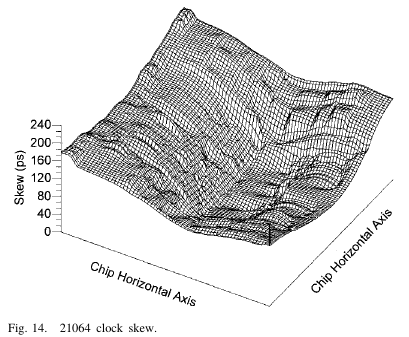
\includegraphics[width=\textwidth]{21064_2.png}
		\caption{clock skew}
	\end{subfigure}
	~ %add desired spacing between images, e. g. ~, \quad, \qquad, \hfill etc. 
	%(or a blank line to force the subfigure onto a new line)
	\begin{subfigure}[b]{0.3\textwidth}
		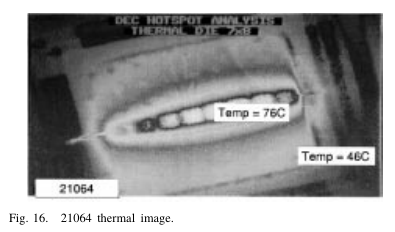
\includegraphics[width=\textwidth]{21064_3.png}
		\caption{thermal imag}
	\end{subfigure}
	\caption{Alpha 21064 clock system analysis (\note{a mouse with teeth, see right most graph})}
\end{figure}
\begin{figure}[h]
	\centering
	\begin{subfigure}[b]{0.3\textwidth}
		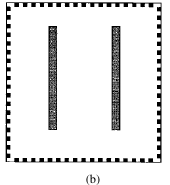
\includegraphics[width=\textwidth]{21164_1.png}
		\caption{clock driver location}
	\end{subfigure}
	~ %add desired spacing between images, e. g. ~, \quad, \qquad, \hfill etc. 
	%(or a blank line to force the subfigure onto a new line)
	\begin{subfigure}[b]{0.3\textwidth}
		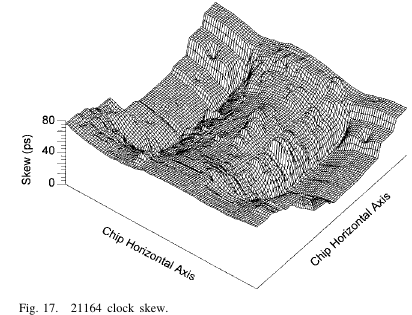
\includegraphics[width=\textwidth]{21164_2.png}
		\caption{clock skew}
	\end{subfigure}
	~ %add desired spacing between images, e. g. ~, \quad, \qquad, \hfill etc. 
	%(or a blank line to force the subfigure onto a new line)
	\begin{subfigure}[b]{0.3\textwidth}
		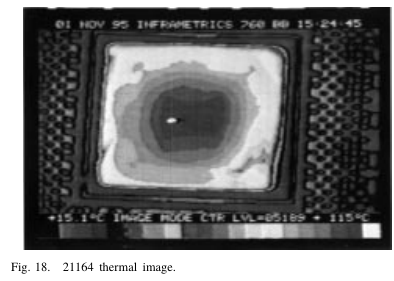
\includegraphics[width=\textwidth]{21164_3.png}
		\caption{thermal imag}
	\end{subfigure}
	\caption{Alpha 21164 clock system analysis}
\end{figure}
From above figures we can see that the nearer clock driver, the lower latency skew and the higher temperature.

And below is the approximate power breakdown of the 21064 and the 21164
\begin{center}
	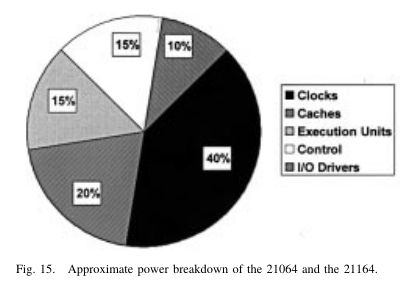
\includegraphics[scale=0.5]{power_consume.png}
\end{center}
It tells us that the clock driver is the main power consumer, consuming 40\% of the chip power.

And as more aggressive circuit techniques and complex micro-architecture features were implemented in the 21264, power consumption became a major concern in designing the clocking system. Thus, new tech was introduced--GCLK to reduce clock grid RC delay and distribute clock power.
\begin{center}
	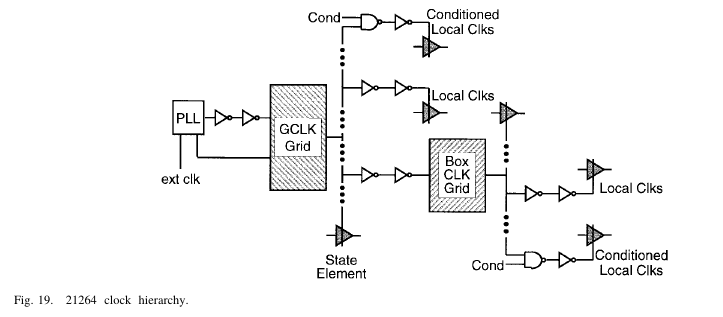
\includegraphics[scale=0.5]{GCLK.png}
\end{center}
So what is GCLK?

GCLK is the root of a hierarchy of thousands of buffered and conditioned local clocks used across the chip as shown in the above picture. There are 2 advantages and 1 dis.
\begin{itemize}
	\item adv: conditioning the local clocks saves power.
	\item adv: circuit designers can take advantage of multiple clocks (\note{for example, a phase path can }).
	\item disad: significantly complicates race and timing verification.
	\item notice: using local buffering significantly lowers the GCLK load, which reduces GCLK skew.
\end{itemize}
\begin{center}
	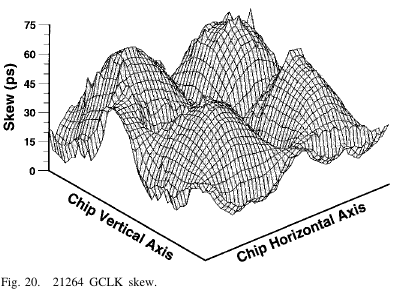
\includegraphics[scale=0.5]{21264.png}
\end{center}
Next part of the paper talks about latch design. Recall my Digital circuit course, I've learned several kinds of latch and flip-flops. Realize it is really a significant element of the microprocessor circuit design strategy. In other word, no latch and flip-flops, no timing logic, no CPU! And as the paper mentioned ``In order to ensure proper operation across all operating conditions, clock and latch circuits cannot designed independently.'' In fact, each generation of the Alpha microprocessor has utilized latches with improved characteristic combined with the improvements to the clock distribution networks previously described.

Thus, the motivation of making low-latency latch design is for high speed. Besides, other primary goals in latch design are minimal area and clock loading, low power dissipation, and low setup and hold times.

Some highlight I've ever seen in general and in each generation of the Alpha microprocessor.
\begin{enumerate}
	\item \textbf{In general} \\
	The capability of embedding a logic function directly in the latch helps reduce the number of gate delays per cycle. (\textbf{Confused}) 
	\begin{center}
		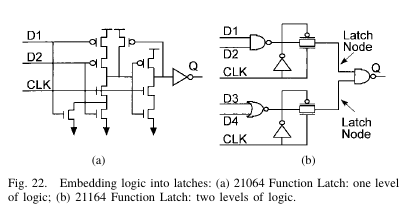
\includegraphics[scale=0.5]{embedding_Latch.png}
	\end{center} 
	the paper says that in some instances, both inverters were replaced with logic gates, further reducing the latching families are show in above graph. It can be seen that the cost of latching in the 21164 could be reduced to a minimum of one pass transistor.
	\item \textbf{21064} \\
	Digital's first microprocessor to use a two-phase, single wire-clocking scheme (\note{this was radical departure from the four-phase scheme that allowed for free design in previous versions of Digital's microprocessors}).
	
	Reducing the chance of data race-through using a variation of the true single-phase clocked (TSPC) level-sensitive latch (an example see below graph).
	\begin{center}
		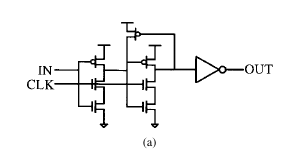
\includegraphics[scale=0.5]{TSPC.png}
	\end{center}
	feature: using the unbuffered main clock directly, significantly increasing race immunity. In addition, the first stage of this latch can incorporate a simple logic function.
	\item \textbf{21164} \\
	using dynastic CMOS transmission gate latch. (an basic example see below graph)
	\begin{center}
		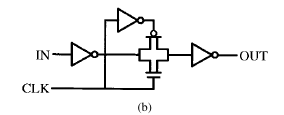
\includegraphics[scale=0.5]{dynamicOMS.png}
	\end{center} 
	feature: requiring true and complementary clock signals, one of which is generated locally.  The clock buffer for each latch type was custom designed so that its delay and edge rate characteristics could be tightly controlled. The additional buffer delays the clocking of the latch by one gate delay after the global clock transitions. (\note{However, since the preceding latch opens with the global clock transition, the possibility of latch race-through is significantly increased. In order to minimize the possibility of data race-through with the use of these latches, at least one minimum logic delay element was required between all latches.})
	\item \textbf{21264} \\
	Requiring a static latch design and using a family of edge-triggered flip-flops, based on the dynamic flip-flop show in following graph.
	\begin{center}
		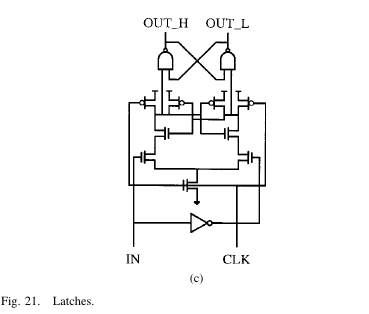
\includegraphics[scale=0.5]{21264_latch.png}
	\end{center} 
	It was developed to simplify the timing and race issues that were exacerbated by the addition of conditional clocking.  The change from level-sensitive to edge-triggered design techniques and the use of multiple clock buffers introduced a number of new timing issues to the design.
\end{enumerate}

Critical path and race analysis

\textbf{Goal}: The capability of buffering and conditioning the main clock is  possible as long as each circuit satisfies both its critical path and race requirements.

What does path and race analysis do? 

it starts with the \textbf{identification of the common clock} initialing \textbf{both the receive and drive paths}, denoted $ R $ and $ D $, Every critical path or race is defined by a \textbf{single common clock and a pair of receive and drive paths}. Here we say the two respective common clocks are GCLK \& FCLK. 
\begin{enumerate}
	\item Critical path analysis \\
	verifies that the difference in delay between the drive path $ D $ plus the receiver setup time and the receive path $ R $ does ont exceed the phase or cycle time of the common clock. For worst case analysis, effects that minimize $ R $ and maximize $ D $ are considered.
	\item Race analysis \\
	Effects that maximize $ R $ and minimize $ D $ are considered. When the ratio of delay of the drive path $ D $ to the receive path $ R $, including hold time, is equal to 1, the circuit is on the verge of failing. Ratios (denoted by X) exceeding 1 imply a margin that may be used to account for effects not included in the analysis. 
\end{enumerate}
\begin{center}
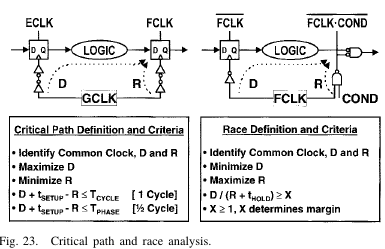
\includegraphics[scale=0.5]{path.png}
\end{center} 
see above graph, the left example illustrates the use of two buffered section clocks, ECLK and FCLK, in a one-cycle path. The circuit on the right of the figure combines a buffered local clock and a conditioned local clock to define a one-phase path.

\textbf{CAD tools and verification}

\textbf{Background}: Commercially available EDA design systems and point CAD tools have very limited support for \textbf{Custom circuit techniques}. Therefore, Digital developed an extensive suite of in-house CAD tools to facilitate the design of custom VLSI microprocessors. 

The internally developed CAD suite includes tools for
\begin{enumerate}
	\item schematic and layout entry
	\item two-state and three-state logic simulation
	\item RTL versus schematic equivalence checking
	\item static timing analysis and race verification
	\item parameter and netlist extraction
	\item electrical analysis and verification
\end{enumerate} 
There are two main parts \begin{itemize}
	\item Electrical Verification
	
	Covers all circuit issues that are not related to logic functionality such as timing behavior, electrical hazards and reliability. The primary goal is to verify that all circuits conform to the project design methodology. 
	
	Some highlight of the tools
	\begin{itemize}
		\item filter out all circuits that can easily be validated while identifying the small number of circuits that may have problems and require additional analysis.
		\item perform over 100 unique electrical checks. and there are three around kinds \begin{itemize}
			\item the major areas of focus are circuit topology violations, dynamic node checks, writeability checks, latch checks, beta ratio checks, gate fan-in \& fan-out restrictions, transistor size and stack height limitations, max/min edge rates and delays, and power consumption.
			\item are applied to all circuit styles
			\item are required for specific circuit types. 
		\end{itemize}
	\end{itemize}
	\item Functional and Logical Verification
	
	Covers all phases of the design process from functional definition through manufacturing tests.
	
	A tow-state RTL behavioral model is the primary verification vehicle.
\end{itemize}

\textbf{Future Challenges}
\begin{enumerate}
	\item power consumption
	\item the distribution of a chipwide timing reference with extremely fast edge rates
\end{enumerate}
\newpage
\section*{2.high logic ``RTL'' aspect\footnote{reading note from \textit{The Alpha 21264 Microprocessor}}}
The first part is mainly about custom circuit design techniques which is the CMOS level design and optimization. However, it is not very suitable for me to do some further works thanks to my poor base of digital circuit. Therefore, I'd like to focus on higher level which is called RTL level or functional logic level. And the design and optimization of this level is much easier to get hands dirty. Therefore, reading this paper is good to begin with my undergraduate thesis. 

Alpha 21264 is a masterpiece in my eyes. It is elaborate designed and has many things to learn from.

This paper discusses two aspect, inner CPU core and outer cache and memory system.
\begin{itemize}
	\item CPU core: A unique combination of high clock speeds and advanced microarchitectural techniques, including many forms of out-of-order and speculative execution
	\item memory system: high-bandwidth memory system that can quickly deliver data values to the execution core (including those without cache locality). 
\end{itemize}

\textbf{Architecture highlights}
\begin{enumerate}
	\item is a superscalar microprocessor that can fetch and execute up to 4 instructions per cycle. It also features out-of-order execution.
	\item employs speculative execution to maximize performance. In other words, when the 21264 predicts branch directions and speculatively executes down the predicted path. With more functional units and these dynamic execution techniques than 21164.
	\item Its memory system also enables high performance levels. On-chip and offchip caches provide for very low latency data access. Additionally, the 21264 can service many parallel memory references to all caches in the hierarchy, as well as to the off-chip memory system.
\end{enumerate}
\begin{center}
	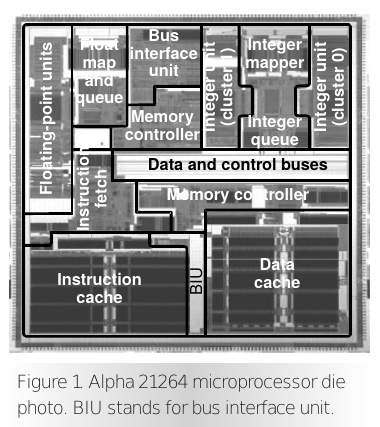
\includegraphics[scale=0.5]{overview.png}
\end{center}
Highlighting major sections of the 21264. We can see that on-chip cache is divided into two--Instruction cache and Dada cache. And it seems like there are the Bus interface unit has two parts, one is in the above and another is in the below. And Instruction fetch is in the middle which is very reasonable for high performance.
\begin{center}
	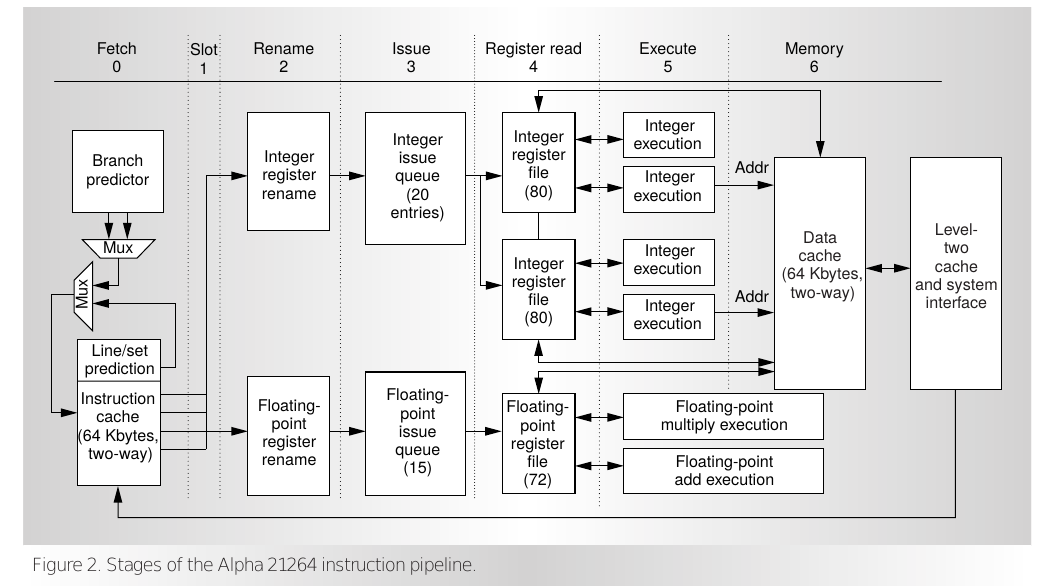
\includegraphics[width=\linewidth]{pipeline.png}
\end{center}
The pipeline is showed above, which has seven stages. One notable addition compared with 21164 is the map stage that renames registers to expose instruction parallelism--this addition is fundamental to the 21264's out-of-order techniques.

And now let's close look at each stage following with the paper.
\begin{itemize}
	\item instruction pipeline--Fetch
	
	Two architectural techniques increase fetch efficiency: line and way prediction and branch prediction. The 21264 has a 64KB, two-way set-associative instruction cache offers much improved level-one hit rates compared to the 8KB, direct-mapped instruction cache in the Alpha 21164.
	\begin{enumerate}
		\item Line and way prediction
		\begin{center}
			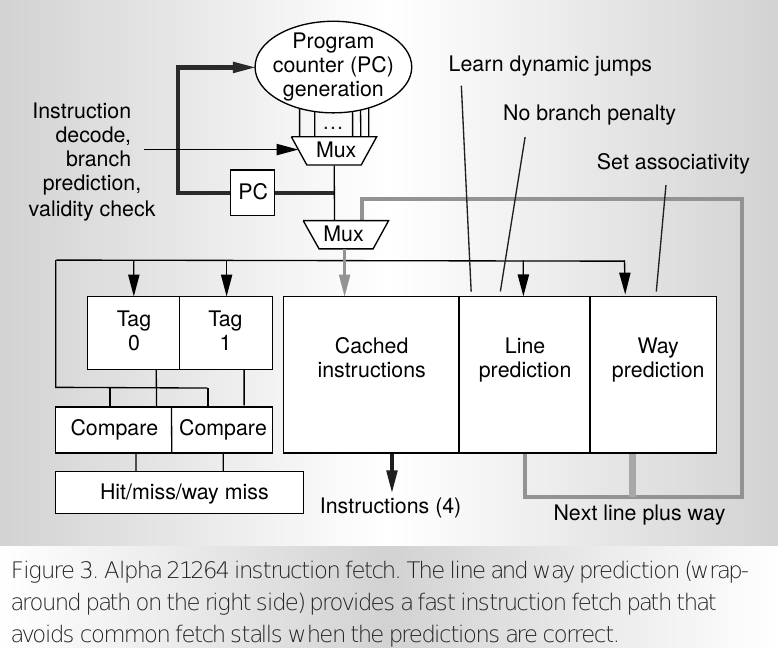
\includegraphics[scale=0.35]{fetch.png}
		\end{center}
		Each 4-instruction fetch block includes a line and way prediction. This prediction indicates where to fetch the next block of 4 instructions, including which way--that is, which of the two choices allowed by 2-way associative cache. As an additional precaution, a 2-bit hysteresis counter associated with each fetch block eliminates overtraining--training occurs only when the current prediction has been in error multiple times (\note{Line and way prediction is an important speed enhancement since the mispredict cost is low and line/way mispredictions are rare}).
		
		Besides, the fetch engine prefetches up to four 64-byte(or 16-instruction) cache lines to tolerate the additional latency.
		\item Branch prediction
		
		The 21164 could accept 20 in-flight instructions at most, but the 21264 can accept 80, offering many more parallelism opportunities. Thus, Branch prediction is more important to the 21264's efficiency than to previous microprocessors. Here are 3 considerations:
		\begin{enumerate}
			\item the 7 cycles mispredict cost is slightly higher than previous generations.
			\item the instruction execution engine is faster than in previous generations.
			\item successful branch prediction can utilize the processor's speculative execution capabilities. 
		\end{enumerate}
		
		The 21264 implements a sophisticated tournament branch prediction scheme. The motivation is that the processor can adapt to dynamically choose the best method for each type of branch. Therefore, the scheme is designed to dynamically choose between two types of branch predictors\begin{itemize}
			\item using local history
			\item using global history
		\end{itemize}
		\begin{center}
			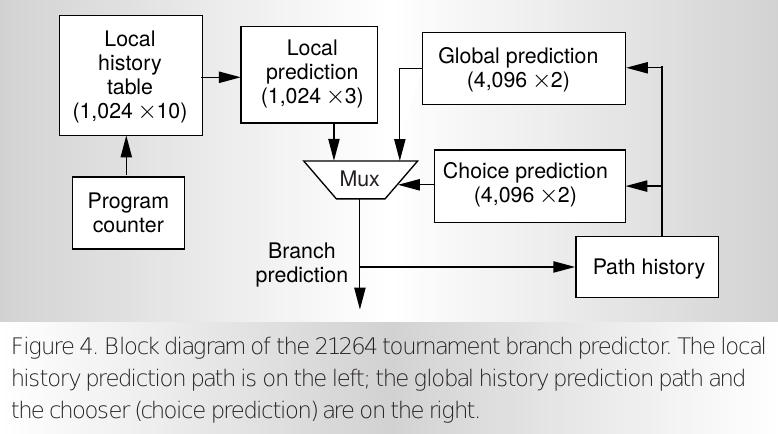
\includegraphics[scale=0.35]{predictor.png}
		\end{center}
	in detailing the structure of the tournament branch predictor, shows 
	\begin{enumerate}
		\item the local history prediction path--through a 2-level structure--on the left. the first level holds 10 bits of branch pattern history for up to 1024 branches. This 10-bit pattern picks from one of 1024 prediction counters.
		\item the global predictor is a 4096-entry table of 2-bit saturating counters indexed by the path, or global, history of the last 12 branches. 
		\item the choice prediction, or chooser, is also a 4096-entry table of 2-bit prediction counters indexed by the path history.
	\end{enumerate} 
	\end{enumerate}
	\item Out-of-order execution
	
	The out-of-order execution logic receives four-instructions every cycle, renames/remaps the registers to avoid unnecessary register dependencies, and queues the instructions until operands or functional units become available.
	
	It dynamically issues up to 6 instructions every cycle--4 integer instructions and 2 floating point instructions.
	\begin{enumerate}
		\item Register renaming
		
		The 21264 speculatively allocates a register to each instruction with a register result. The register only becomes part of the user-visible (architectural) register state when the instruction retires/commits.
		
		Register renaming also eliminates write-after-write and write-after-read register dependencies, but preserves all the read-after-write register dependencies that are necessary for correct computation.
		\begin{center}
			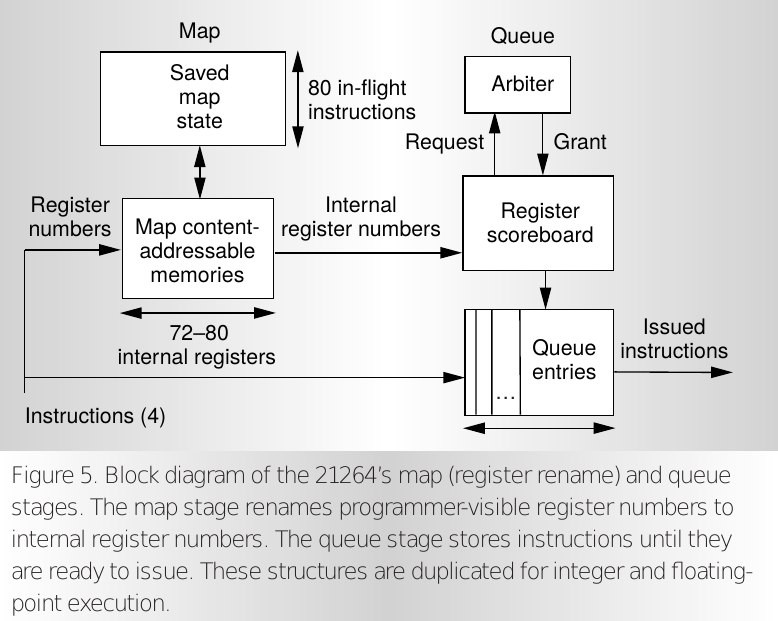
\includegraphics[scale=0.35]{rename.png}
		\end{center}
		Register renaming is a content-addressable memory (CAM) operation for register sources together with a register allocation for the destination register.
		
		Beyond the 31 integer and 31 floating-point user-visible (non-speculative) registers, an additional 41 integer and 41 floating-point registers are available to hold speculative results prior to instruction retirement.
		\item Out-of-order issue queues
		
		There are tow components. One is the queue logic itself which maintains two list of pending instructions in separate integer and floating-point queues. Anther is register scoreboards based on the internal register numbers. 
		
		\textbf{How scoreboards works?}
		
		These scoreboards maintain the status of the internal register by tracking the progress of single-cycle, multiple-cycle, and variable-cycle (memory load) instructions. When functional-unit or load-data results become available, the scoreboard unit notifies all instructions in the queue that require the register value. These dependent instructions can issue as soon as the bypassed result becomes available from the functional unit or load.
		
		The 20-entry integer queue can issue for 4 instructions and the 15-entry float-point queue can issue 2 instructions per cycle.
		\item Instruction retire and exception handling
		
		The 21264 implements a precise exception model using in order retiring, which means that the programmer does not see the effects of a younger instruction if an older instruction has an exception.
		
		From issue until retire eligibility, how many cycles will take for each instruction? Well, it is up to the classes of instructions. \begin{enumerate}
			\item Integer inst needs at least 4 cycles.
			\item Memory access inst needs at least 7 cycles.
			\item Floating-point inst needs at least 8 cycles.
			\item Branch/jump to subroutine inst needs at least 7 cycles.
		\end{enumerate}
	
		Besides, the retire mechanism can retire at most 11 instructions in a single cycle, and it can sustain a rate of 8 per cycle (over short periods).
	\end{enumerate}
	\item Execution engine
	\begin{center}
		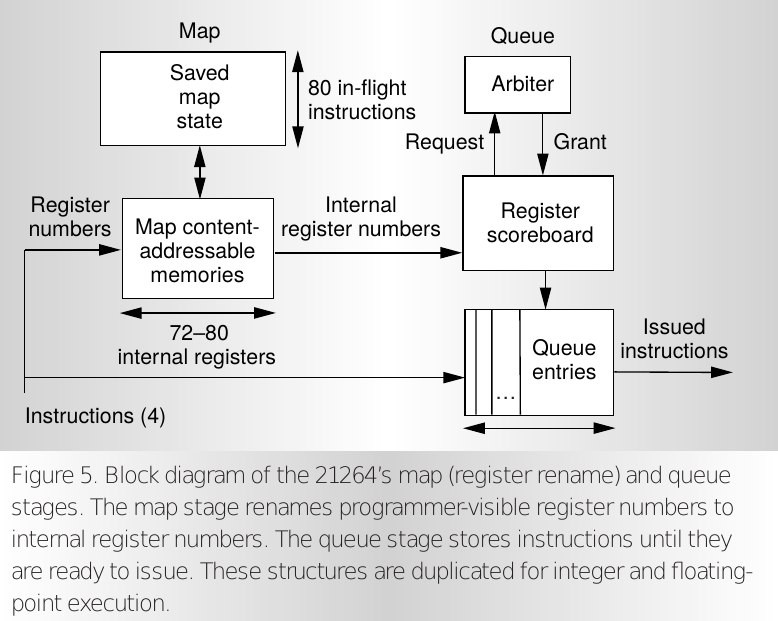
\includegraphics[scale=0.35]{rename.png}
	\end{center}
	\textbf{a bit of confused for the above graph}
	
	The clusters is a special design in my opinion. How it works? Two pipes access a single register file to form a cluster, and the two clusters combine to support four-way integer instruction execution. This clustering makes the design simpler and faster, although it costs an extra cycle of latency to broadcast results from an integer cluster to the other cluster. Other thing need to pay attention is that The upper pipelines from the two integer cluster are managed by the same issue queue arbiter, as are the tow lower pipelines. By the way, this part is still hard to understand until to implement by myself.
	\item \emphasize{Internal memory system (\textbf{this part is extremely important, need more time to digest, and use these techniques in my own CPU memory system })}
	
	It is a high-band-width, low-latency memory system.
	
	Here are several features: \begin{enumerate}
		\item service up to 2 memory references from the integer execution pipes every cycle. These 2 references are out-of-order issues.
		\item simultaneously tracks up to 32 in-flighting loads, 32 in-flighting stores, and 8 in-flighting (instruction or data) cache misses.
		\item also has a 64KB, two-way set-associative data cache.
	\end{enumerate}
	\begin{enumerate}
		\item Data path
		
		The 21264 supports any combination of two loads/stores per cycle without conflict. How to achieve it? The data cache is double-pumped with two-ports and operates at twice the frequency of the processor clock -- an important feature of the 21264's memory system.
		\begin{center}
			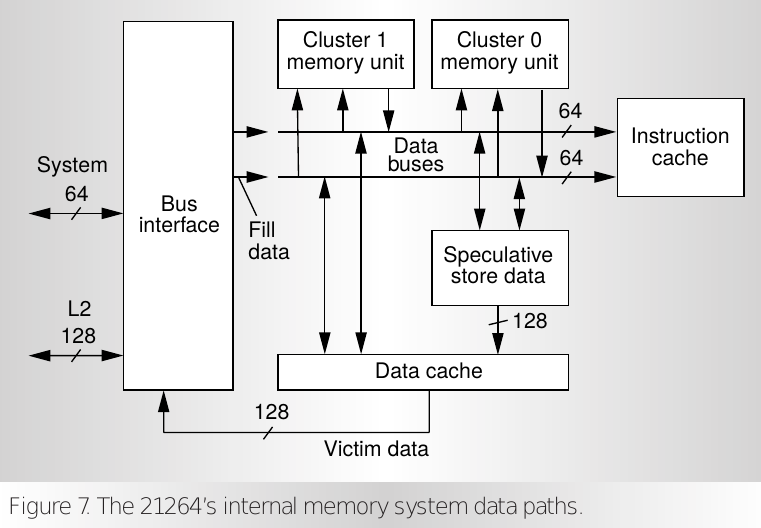
\includegraphics[scale=0.35]{dataPath.png}
		\end{center}
		The 2 64-bit data buses are the heart of the internal memory system. Let's consider two operations -- load and store
		\begin{itemize}
			\item load: there are three sources can load data from: \begin{itemize}
				\item the data cache
				\item the speculative store data buffers
				\item an external (system or L2) fill
			\end{itemize}
			\item store: First transfer their data across buses into the speculative store buffer until the stores retire. Once they retire, the data is written (dumped) into the data cache on idle cache cycles. Each dump can write 128 bits into the cache since two stores can merge into one dump.
		\end{itemize}
		The optimization of load and store if we consider them together:
		
		Stores can forward their data to subsequent loads while they reside in the speculative store data buffer. Load instructions compare their age and address against these pending stores. On a match, the appropriate store data form the data cache. In effect, the speculative store data buffer performs a memory-renaming function. From the perspective of younger loads, it appears the stores into the data cache immediately. (\note{also some further details but not fully understand: Fill data arrives on the data buses. Pending loads sample the data to write into the register file while, in parallel, the caches (instruction or data) also fill using the same bus data. The data cache is write-back, so fills also use its double-pumped capability: The previous cache contents are read out in the same cycle that fill data is written in. The bus interface unit captures this victim data and later writes it back.})
		\item Address and control structure
		
		The internal memory system maintains a 32-entry load queue (LDQ) and a 32-entry store queue (STQ) that manage the references while they are in-flight. The LDQ(STQ) positions loads(stores) in the queue in fetch order, although they enter the queue when they issue, out of order. Loads exit the LDQ in fetch order after the loads retire and the load data has been returned. Store exit the STQ in fetch order after they and dump into the data cache. New issues check their address and age against older references. Dual-ported address CAMs resolve the read-after-read, read-after-write, write-after-read and write-after-write hazards inherent in a fully out-of-order memory system. 
		(\note{For instance, to detect memory read-after-write hazards, the LDQ must compare addresses when a store issues: Whenever an older store issues after a younger load to the same memory address, the LDQ must squash the load -- the load got the wrong data}) The STQ CAM logic controls the speculative store data buffer. It enables the bypass of speculative store data to loads when a younger load issues after an older store.
		\begin{center}
			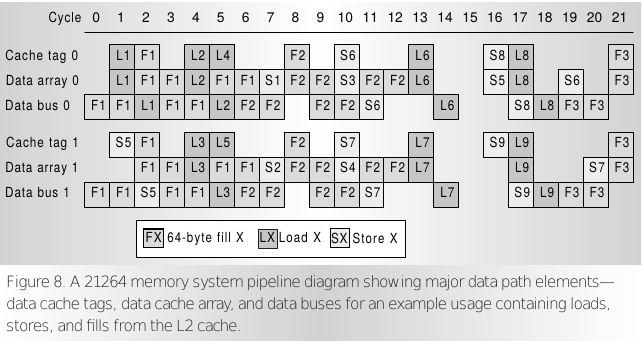
\includegraphics[width=\linewidth]{timing_logic_graph.png}
		\end{center}
		From the above graph, we can see that \begin{itemize}
			\item loads reference both the data cache tags and array in their pipeline stage 6, and then the load result uses the data bus one cycle later in their stage 7.
			\item Stores are similar to loads except they do not use the cache array until they retire.
			\item Fill patterns can get skew between different cycle.
			\item two stores that merge into a single cache dump. And Cache dump can happen when only stores issue. 
			\item Two loads can only use the cache tags, which decouple the cache tag lookup from the data array and data bus use, taking advantage of the data cache tags during fills. This decoupling is particularly useful for loads that miss in the data cache, since in that case the cache array lookup from the data array and data bus transger of the load issue slot are avoid. 
		\end{itemize}
		the last two features introduced in this part are MAF (miss address file) and the fact that the Alpha memory model is weakly ordered. Ordering among references to different memory addresses is required only when the programmer inserts memory barrier instructions.
		\item Cache prefetching and management
		
		The system implements cache prefetch instructions that let the programmer take full advantage of the memory system's parallelism and high-bandwidth capacities (pretty useful in application with loops that reference large arrays). If software can predict memory references, it can prefetch the associated 64B cache blocks to overlap the cache miss time with other operations. 
		\begin{center}
			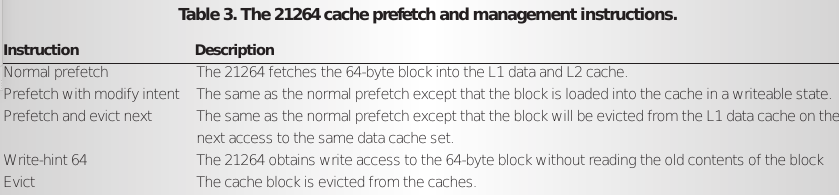
\includegraphics[width=\linewidth]{instruction.png}
		\end{center}
	\end{enumerate}
	\item Bus interface unit
	
	The 21264 bus interface unit (BIU) interfaces the internal memory system and the external (off-chip) L2 cache and the rest of the system. It receives MAF references from the internal memory system and responds with fill data from either the L2 cache on a hit, or the system on a miss. It forwards victim data from the data cache to the L2 and from the L2 to the system using an eight-entry victim file.
	
	\textbf{Attention: the 21264 implements a write-invalidate cache coherence protocol to support shared-memory multiprocessing.}
	\begin{center}
		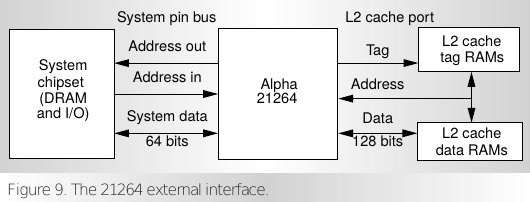
\includegraphics[scale=0.5]{BIU.png}
	\end{center}
	All interconnects on and off the 21264 are high-speed point-to-point channels. They use clock-forwarding technology to maximize the available bandwidth and minimize pin counts (\textbf{confused: what is pin counts}).
	\begin{enumerate}
		\item The L2 cache provides a fast backup store provides a fast backup store for the primary caches. This cache is direct-mapped, shared by both instructions and data, and can range form 1 to 16 MB. However, the BIU is not bind to particular L2 cache. In fact, it can support a wide range of SRAM part variants for different size, speed, and latency L2, including late-write synchronous, PC-style, and dual-data for very high speed operation. 
		\item interface to the system. The 21264 has split address-out and address-in buses in the system pin bus. This provides bandwidth for new address requests (out from the processor) and system probes(into the processor), and allows for simple , small-scale multiprocessor system designs. The 21264 system interface's low pin counts and high bandwidth let a high-performance system (of four or more processors) broadcast probes without using a large number of pins. The BIU stores pending system probes in an eight-entry probe queue before responding to the probes, in order. It responds to probes very quickly to support a system address bus bandwidth required in common probe response cases.
	\end{enumerate}
	 \textbf{Attention: The 21264 provides a rich set of possible coherence actions; it can scale to larger-scale system implementations, including directory-based systems. It supports all five of the standard MOESI(modified-owned-exclusive-shared-invalid) cache states}
	 
	 The BIU supports a wide range of system data bus speeds. Bandwidth, load latency and parallelism.
	\item Dynamic execution examples
	
	what is dynamic execution? The point lies in ``dynamic''. The line predictor, branch predictor, and issue queue scheduling are all representing dynamic principle. Here are two further dynamic adaptability example.
	\begin{enumerate}
		\item Store/load memory ordering
		\item Load hit/miss prediction
	\end{enumerate}
\end{itemize}
\end{document}

